
\chapter{Evaluation}

\section{Benchmarking Environment}

The benchmarking environment involves a single machine that contains a quad-core Intel Xeon Processor L5420 (2.5 GHz) and 16 GBs of RAM. In order to alleviate disturbance of a running measurement and minimize the noise in the results, a bare metal 64-bit Ubuntu 14.04.2 LTS was installed. Additionally, Oracle JDK version 1.7.0 was used as the Java environment.

\section{Benchmark Configuration}

\paragraph{Topologies}

We generate 5 topologies for the measurements such as the scale-free model, hierarchical network and three Watts-Strogatz models by adjusting the its probability $p$ value to $0.1$, $0.01$ and $0.001$. Due to these configurations of $p$, we reach a deviation between Watts-Strogatz models and random graphs.\\ The topologies are generated via our uniform model generation approach (\ref{sec:uniform_generation}).
Every topology is generated 5 times with different densities. The densities are adjusted to 5 different values based on the size of complete graphs in the hierarchical network. The $K_n$ complete graphs are configured to $K_3$, $K_4$, $K_5$ $K_6$ and $K_7$.

\paragraph{Queries}
The queries are parameterized and executed 20 times in a sequence.

\section{Samples}

In order to analyze the relationships between model metrics and performance of query evaluations, we create different samples of the measurements and investigate them respectively. The triple of a tool, query and a specific model size (number of nodes) defines a sample indicating that it includes the measurement results of one particular query per a tool based on a certain size of the models. As a result, the number of different samples is equal to the product of unique tools, queries and model sizes.

\subsection{Sample Size}
A sample includes the measurements executed on 5 different topologies, and each of them appears 5 times in the sample with different density that are configured between the various topologies equally. In other words, . The densities are determined by the hierarchical network topology, as we use different size of $K_n$ complete graphs in its generation algorithm, namely, $K_3$, $K_4$, $K_5$ $K_6$ and $K_7$.\\
One sample contains 20 evaluations of a parameterized query. Finally, the dimensions in a sample and their occurrences are illustrated in Table \ref{tab:sample_size}. As it can be observed, the sample size is equal to $500$.

\begin{table}[ht]
	\footnotesize
	\centering
	
	\begin{tabular}{ l c c c c c c || c }
		\toprule
		 & Tool & Query & Model Size & Query Evaluation & Topology  & Density & $\prod$\\ [5pt] \hline
%		\midrule 
		Occurrence & 1 & 1 & 1 & 20 & 5 & 5 & 500 \\ \hline
		\bottomrule
	\end{tabular}
	\caption{The dimensions and their occurrence in a sample.}
	\label{tab:sample_size}
\end{table}



\section{How to Read the Charts}

\section{Model Analysis}

\subsection{Density}
One essential expectation was in our work to generate different graphs with the same number of nodes and edges. Figure \ref{fig:density} depicts the density of the topologies. The X-axis represents the sizes of the models, the Y-axis shows the value of the metric density. Every column contains the information of one specific topology, furthermore, the different densities are separated by colours in the legend.
\begin{figure}[!ht]
	\centering
	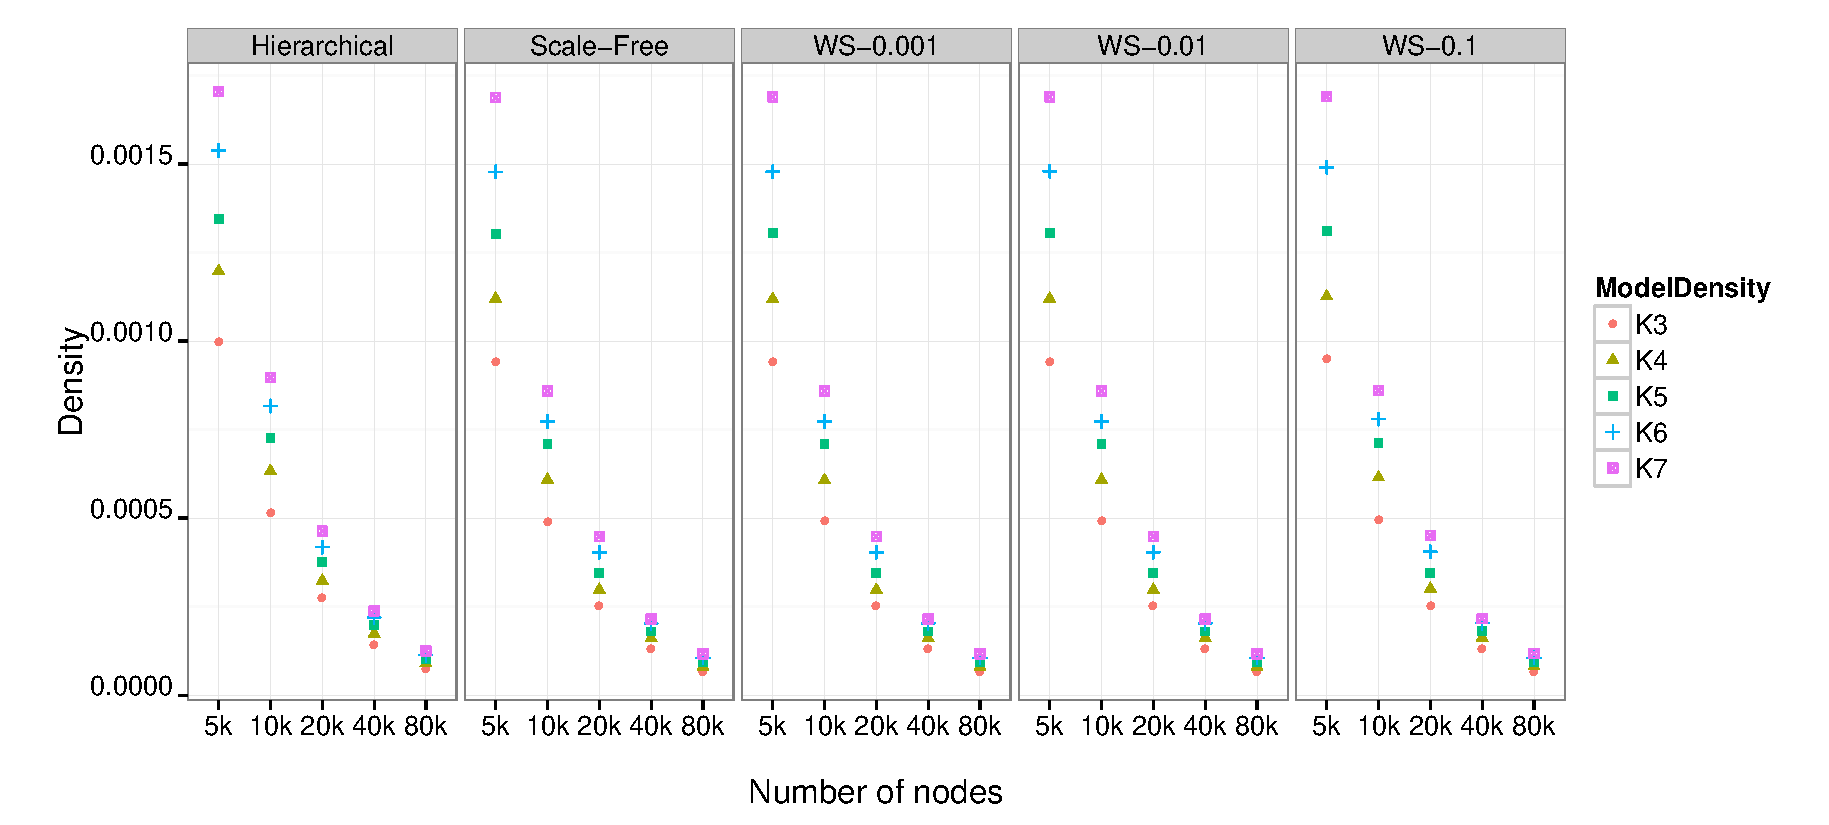
\includegraphics[width=160mm, keepaspectratio]{figures/density.pdf}
	\caption{The density of the graph topologies.}
	\label{fig:density}
\end{figure}

As it can be observed, the topologies with different networks have approximately the same density with the respect to the number of nodes, which implies an equality in the number of edges. A small deviation is showed between the hierarchical graph and the other topologies due to the fact that the recursive generation algorithm of the former must be terminated before its end to obtain an arbitrary number of nodes, hence, we can only estimate the amount of edges in the graph with a small deviation.

\subsection{Clustering Coefficient}

Our goal is to achieve a deviation in metric values per topologies such as the clustering coefficient metric. Figure \ref{fig:clustering_metric} depicts the average clustering coefficients in the topologies. The X-axis represents the number of nodes in the graphs, the Y-axis denotes the values of the metric, furthermore, every value is separated by the topology in legend.\\
The plot shows how the values spread in the $0-1$ interval according to our early expectation (Section \ref{sec:topology_metric}). One topology has more corresponding metric value in the same size---\eg hierarchical---due to the fact that we generated 5 instances of every topology with different densities, which implies a different clustering coefficient metric per instance as well.

\begin{figure}[!ht]
	\centering
	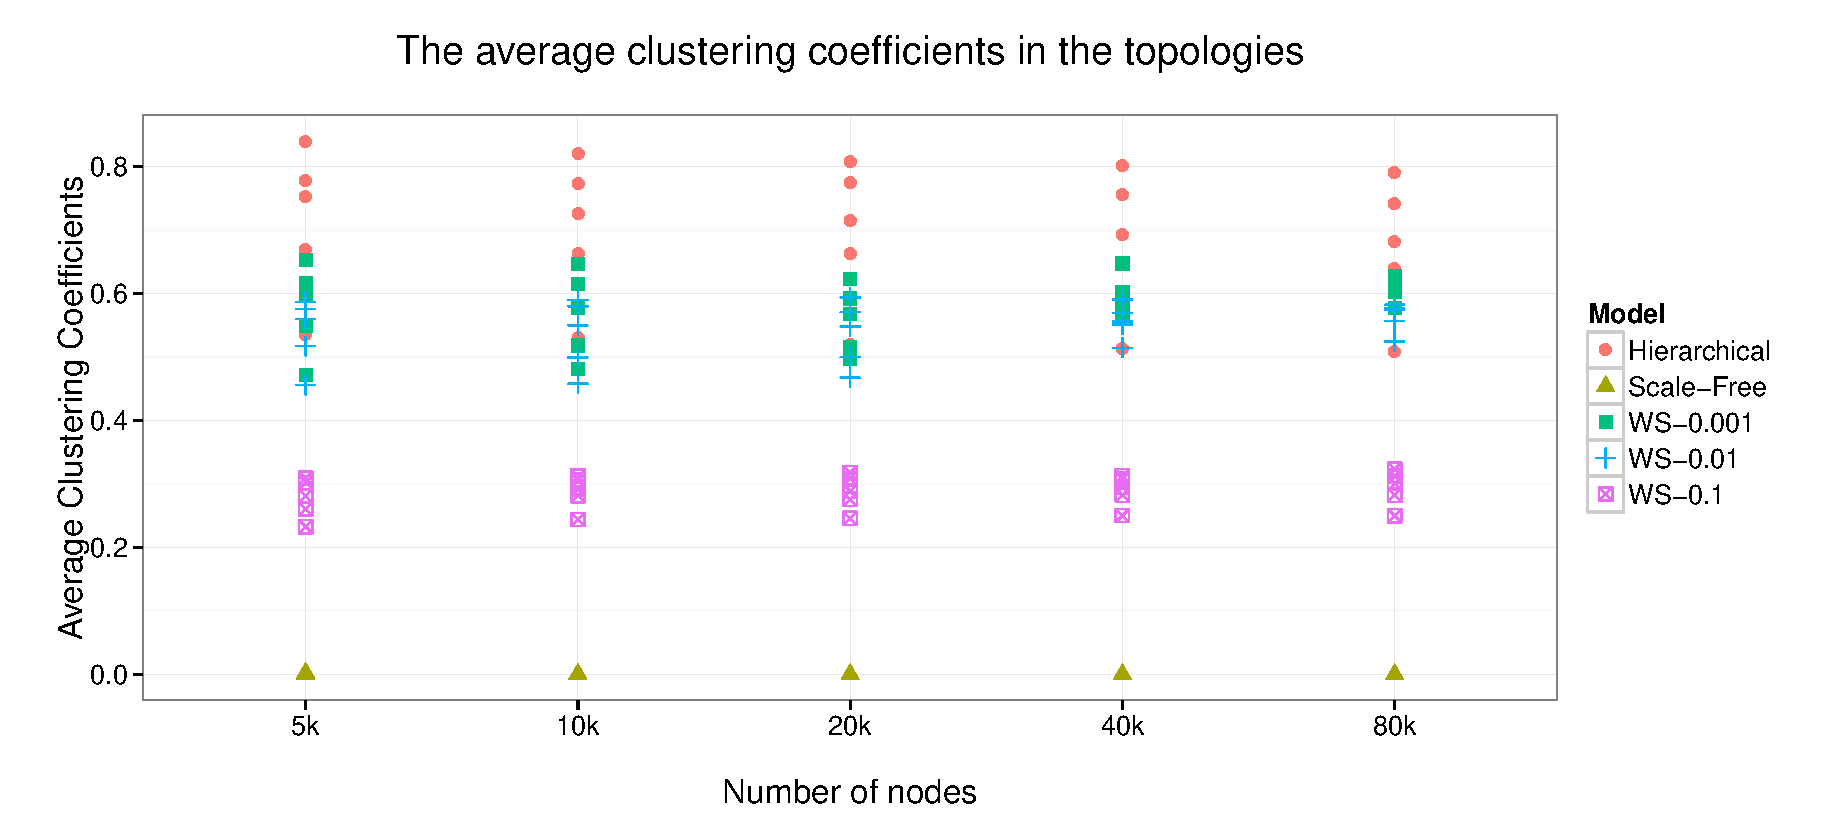
\includegraphics[width=160mm, keepaspectratio]{figures/clustering_metric.pdf}
	\caption{The average clustering coefficient in the graph topologies.}
	\label{fig:clustering_metric}
\end{figure}

\subsection{Shortest Path Length}

The average lengths of shortest paths in the topologies are demonstrated in Figure \ref{fig:betweenness_metric}. Easy to observe that as we decrease the $p$ probability in the Watts-Strogatz models (from $0.1$ to $0.001$) , the lengths of shortest paths increase. This negative correlation shows the results that we expected and can be explained by the construction of the generation algorithm belonging to the Watts-Strogatz model. As we increase the $p$ value, the algorithm rewire every edge with $p$ probability---so it deletes an edge and connects it to a new random node---and this entails a bigger interconnectivity in the graph showing the small-world property. On the contrary, a low $p$ value (\eg 0.001) modifies a subtle set of the edges, therefore, the graph sill shows similar characteristics than a lattice graph with high average shortest path length.

\begin{figure}[!ht]
	\centering
	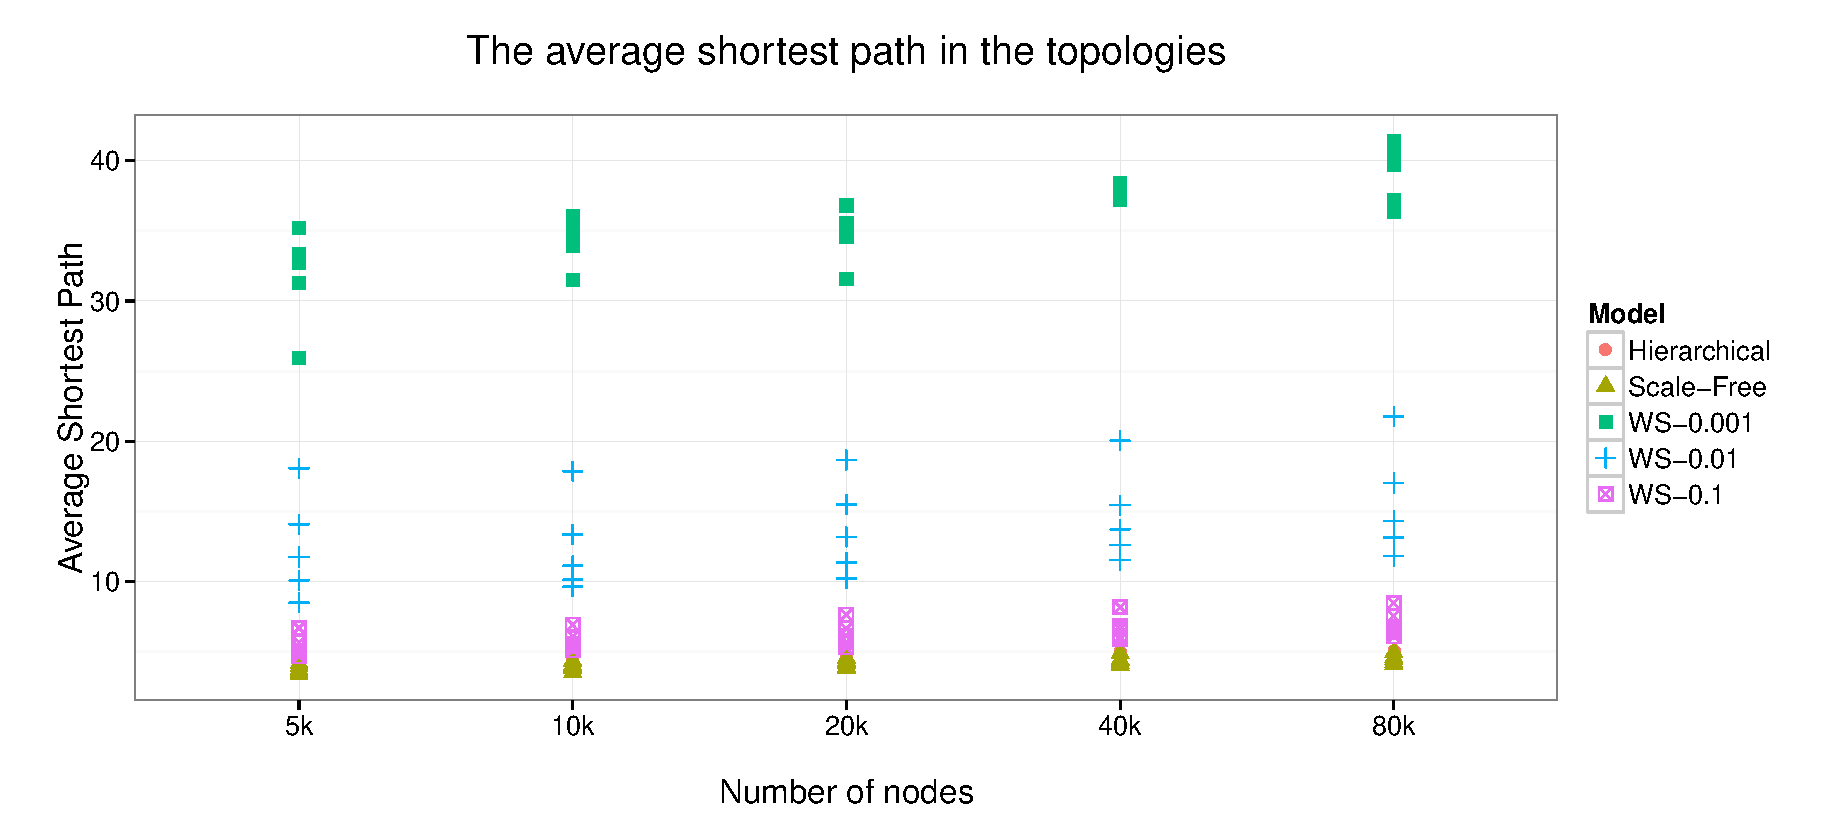
\includegraphics[width=160mm, keepaspectratio]{figures/avg_sp_metric.pdf}
	\caption{The average shortest path in the graph topologies.}
	\label{fig:avg_shortest_path}
\end{figure}

\subsection{Betweenness Centrality}

Figure \ref{fig:betweenness_metric} illustrates the betweenness centrality metric per topologies. Regarding this metric, we assumed a more significant deviation among the topologies, as we expected that the \emph{hubs}---the nodes with higher degrees---in scale-free models appear more in the shortest paths, implying a higher betweenness centrality. Instead, the WS-0.001 model shows higher values in this metric than the scale-free model expect in the largest graph.\\
A gap is observed between the hierarchical network and the other topologies due to the fact the center node in the hierarchical graph dominates the calculation of the betweenness centrality metric.

\begin{figure}[!ht]
	\centering
	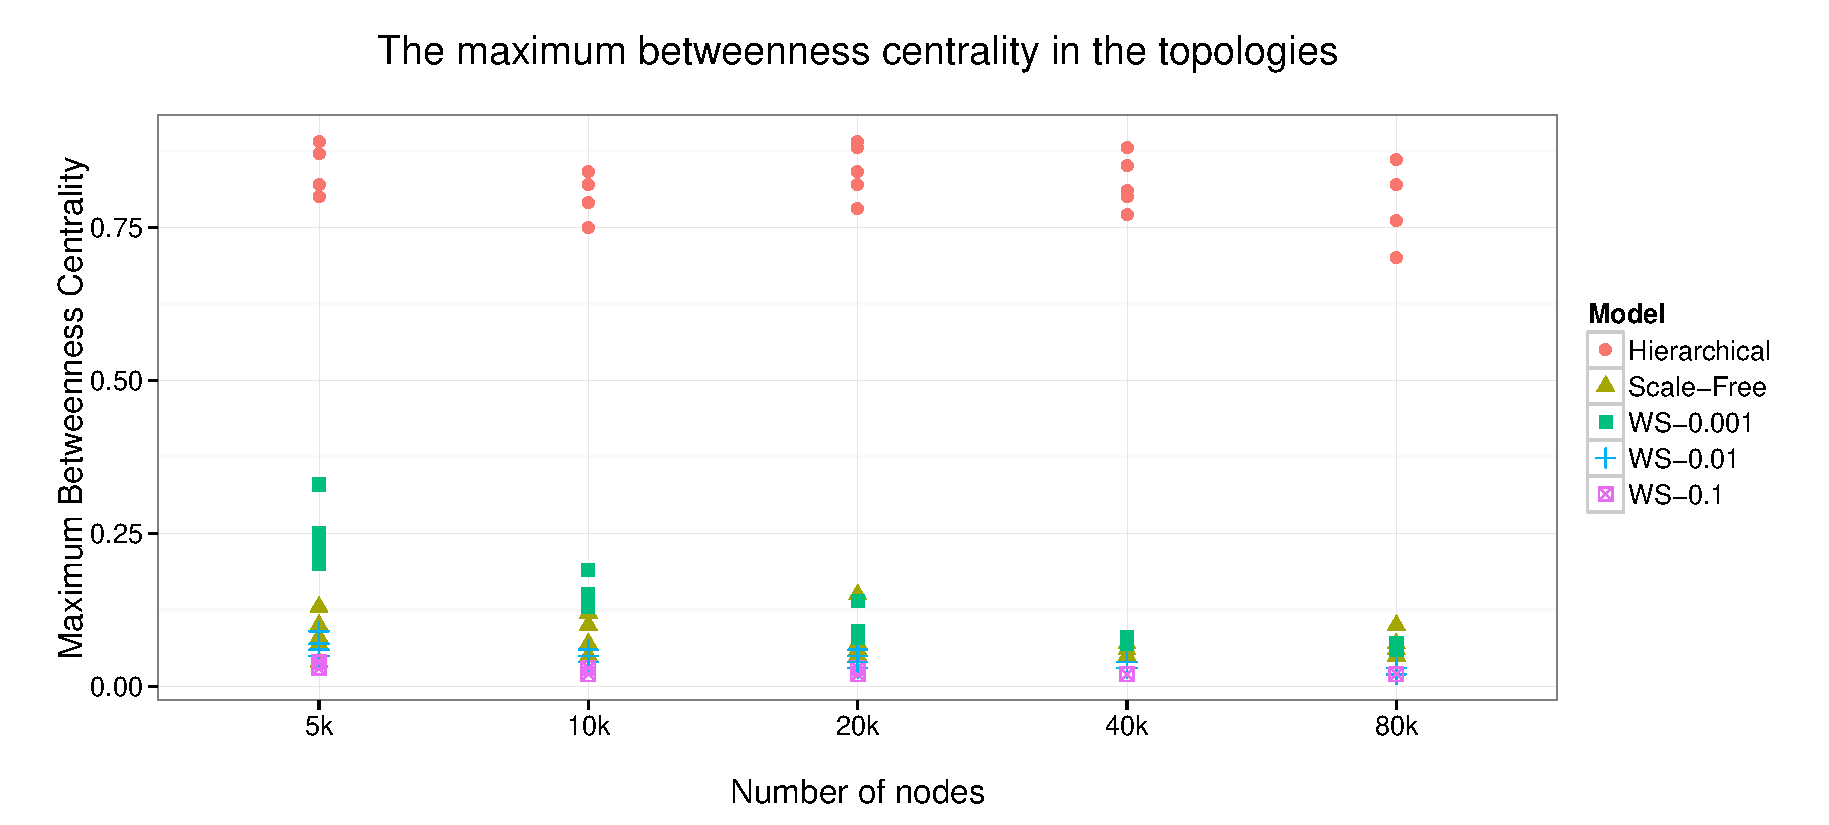
\includegraphics[width=160mm, keepaspectratio]{figures/betweenness_metric.pdf}
	\caption{The maximum betweenness centrality in the graph topologies.}
	\label{fig:betweenness_metric}
\end{figure}



%\begin{tabular}{l l r c c}
%	\hline
%	& \multicolumn{2}{c}{$5000$} \vline & \multicolumn{2}{c}{$5000$} \\
%	\cline{1-2}
%	   & $SD$ & $SD / MAX$ \\
%	\hline
%	$K_3$      & per gram    & 13.65      \\
%	$K_4$ & each        & 0.01       \\
%	$K_5$ & stuffed     & 92.50      \\
%	$K_6$ & stuffed     & 33.33      \\
%	$K_7$ & frozen      & 8.99       \\
%	\hline
%\end{tabular}

\section{Performance Analysis}

\subsection{Hypothesis}

\subsection{Path Query}

An overall plot is showed in Figure \ref{fig:query1} representing the measurement results of the \textsf{Path} query. The evaluation times are showed in milliseconds on the Y-axis with respect to the topology (X-axis) and the size of the model (columns). Every row includes the measurement results provided by a specific tool.

The first important observation is the variation of evaluation times of Blazegraph. The Watts-Strogatz models cause significantly different evaluation time in every model size, additionally, a deviation is also observable between the hierarchical and scale-free networks. As far as the other tools are concerned, Allegro shows a small dispersion in the largest size ($80~000$ nodes), however, Sesame provides an equal evaluation time among the topologies. 

\begin{figure}[!ht]
	\centering
	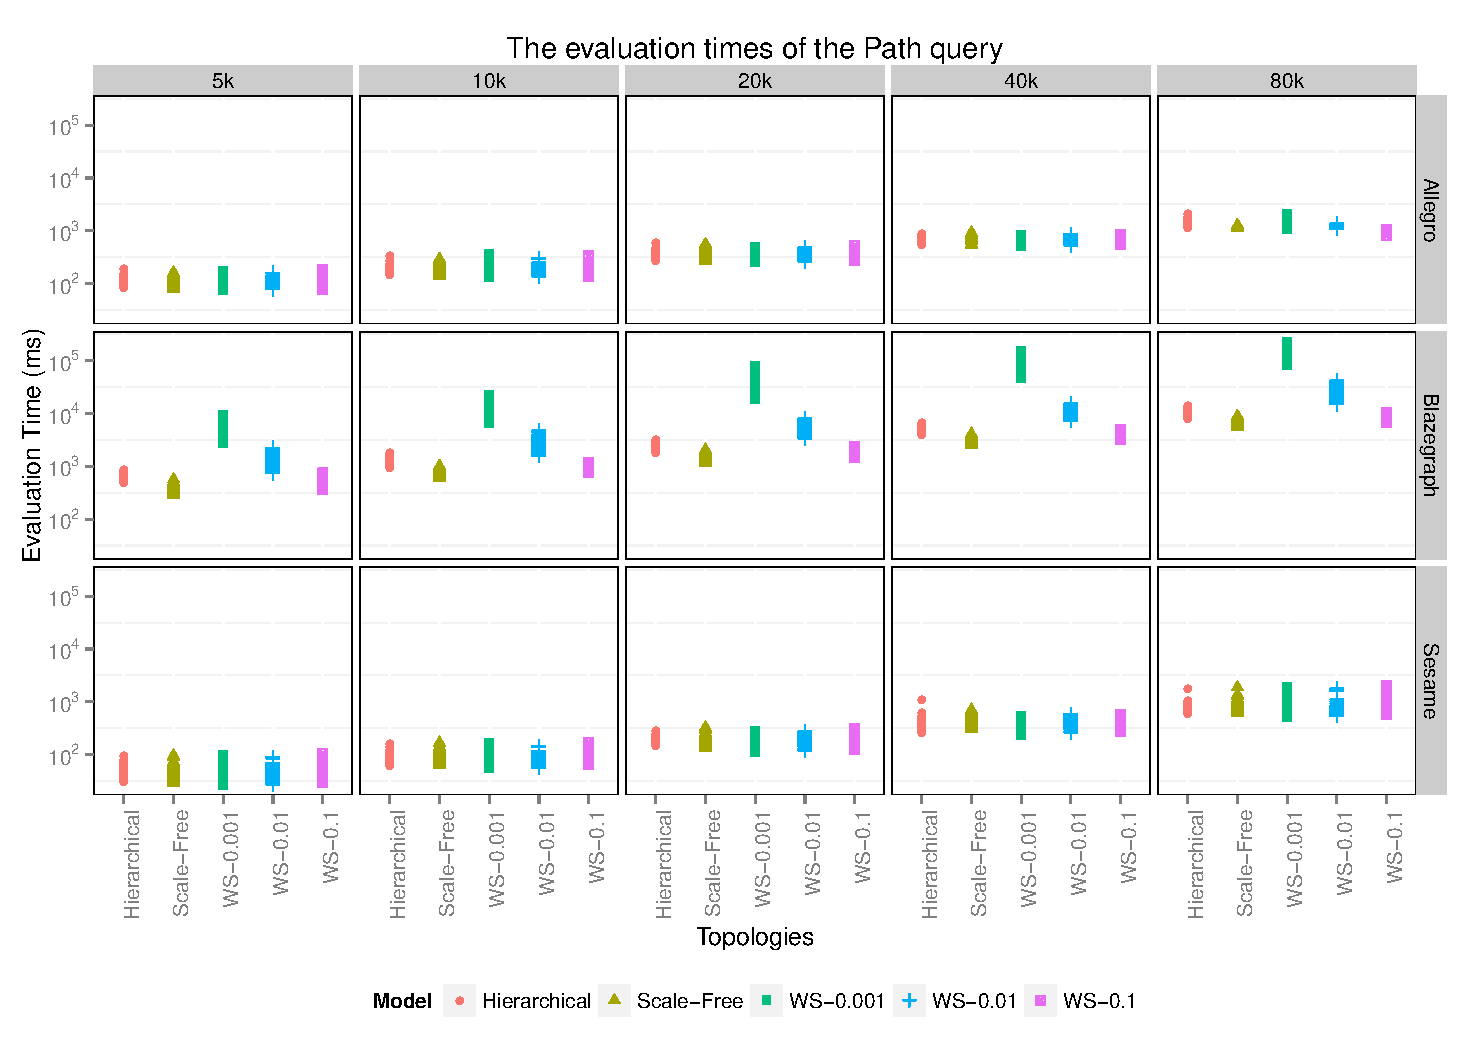
\includegraphics[width=160mm, keepaspectratio]{figures/query1_all.pdf}
	\caption{The measurement results of the Path query.}
	\label{fig:query1}
\end{figure}


\subsubsection{Analyzing Blazegraph}

The measurements result of Blazegraph is illustrated in more details in Figure \ref{fig:blazeq1}.
\begin{figure}[!ht]
	\centering
	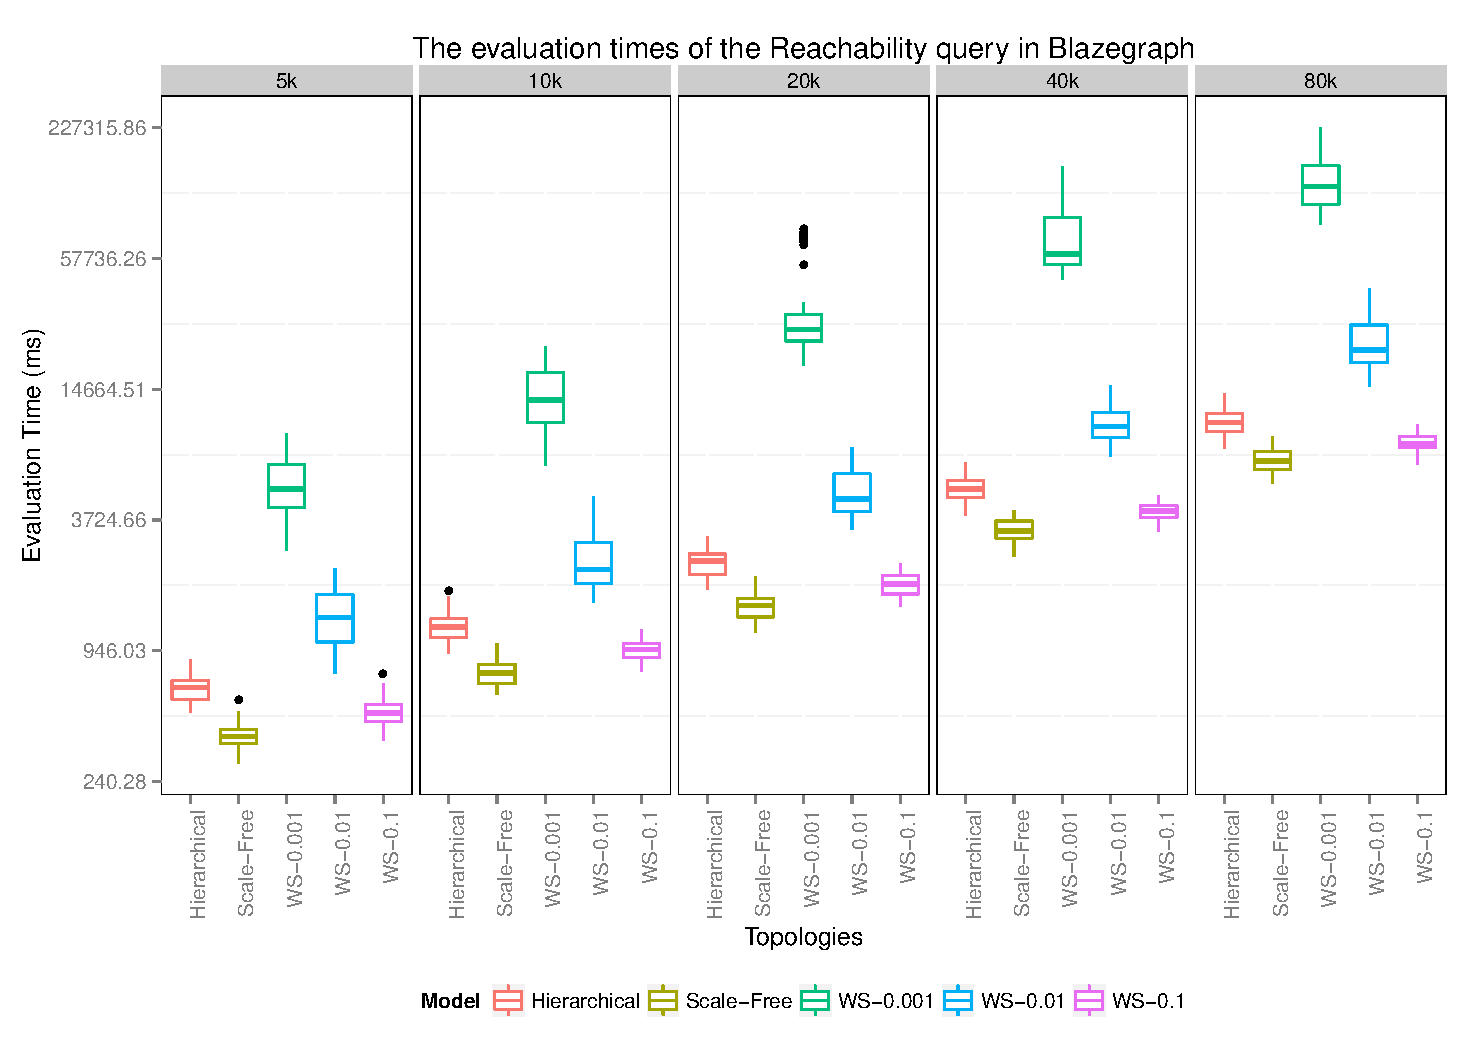
\includegraphics[width=160mm, keepaspectratio]{figures/blaze_q1.pdf}
	\caption{The measurement results of the Path query in Blazegraph.}
	\label{fig:blazeq1}
\end{figure}

\begin{table}[ht]
	\footnotesize
	\centering
	
	\begin{tabular}{ l c c c}
		\toprule
		Metrics & Adjusted R$^2$ Squared & Coefficients & P-values\\ \hline
		%		\midrule 
		Edges & $0.0211$ & $6.5 \cdot 10^{-4}$ \\ 
		Clustering & $0.08532 $ & $1.635 \cdot 10^{-11}$ \\ 
		Betweenness & $0.01616$ & $0.004414$ \\ 
		Avg Shortest Path & \textbf{0.8589} & $2.2 \cdot 10^{-16}$ \\ 
		Avg Shortest Path $+$ Clustering & 0.8589 & Sp: $2.2 \cdot 10^{-16}$; C: 0.157\\ 
		Avg Shortest Path + Betweenness & \textbf{0.8656} & Sp: $2.2 \cdot 10^{-16}$; B: $2.94 \cdot 10^{-7}$ \\
		
		\bottomrule
	\end{tabular}
	\caption{.}
	\label{tab:regressions_blaze_a1}
\end{table}

5k: avg sp:  0.9 p-value: < 2.2e-16 rc: 9.492e-01, in: 4.808e-16
10k: avg sp:  p: 2e-16  rc: 9.268e-01 Adjusted R-squared:  0.8586 
20k: avg sp:  rs: 0.6807 

\begin{figure}[!ht]
	\centering
	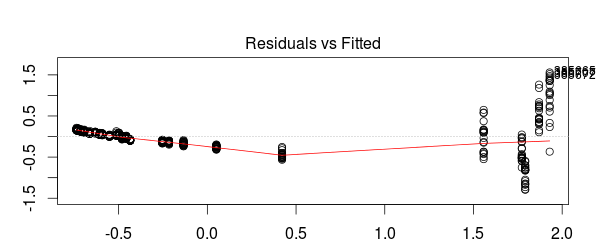
\includegraphics[width=160mm, keepaspectratio]{figures/residuals_blaze_q1.png}
	\caption{.}
	\label{fig:residual_blaze_q1}
\end{figure}

\section{Conclusions}